\chapter{Evaluation}

\begin{figure*}
    \centering
    \small
     \begin{tabular}{l|c|r|l}
       \bf Application        & \bf Type    & \bf LoC & \bf Policies   \\
      \hline
       Atomic~\cite{atomic} (v0.34.2)       & Graph DB    & 9.6k   & Access Control                                 \\
       Contile~\cite{contile} (v1.11.0)     & Advertising & 4.9k     & Purpose Limitation                           \\
       Freedit~\cite{freedit} (v0.6.0-rc.3) & Social      & 6.6k     & Data Retention/Expiration                     \\
       Hyperswitch~\cite{hyperswitch} (v0.2.0)   & Payments    & 198.9k     & Credential Security, Limited Data Collection  \\
       Lemmy~\cite{lemmy} (v0.16.6)        & Social      & 31.4k   & Access Control                               \\
       Plume~\cite{plume} (v0.7.2)         & Blogging    & 21.4k   & Data Deletion                                \\
       WebSubmit~\cite{websubmit} (v1.0)       & Homework    & 1.6k    & Data Deletion, Access Control     \\
    \end{tabular}
    \caption{Case study applications with code size and policies.}
    \label{f:apps}
   \end{figure*}

We evaluate \syslang{} against seven third-party Rust applications to answer four questions:
%
\begin{enumerate}[nosep]
    \item What is the developer effort required to encode policies in \syslang? (\S\ref{sec:accessibility})
    \item Can \syslang's grammar express real-world \policies? (\S\ref{sec:expressivity})
    \item How do \syslang's abstractions impact policy precision and correctness?(\S\ref{sec:precision})
    \item Are \syslang's policies efficient enough for practical use? (\S\ref{sec:efficiency})
\end{enumerate}
%

We tried to pick popular applications spanning different policy domains.
%
We summarize the applications in~\Cref{f:apps}.

\section{Developer Effort}
\label{sec:accessibility}
%
We evaluate the effort required to encode policies in \syslang{}.
%
For each application, we had two groups write policies.
%
The first group wrote the policies using the Graph Query API, while the other used \syslang{}.
%
The Graph Query API group simulated the process of an application \dev{} who decided on policies by referencing application source code.
%
The \syslang{} group emulated the role of a \ce{}.
%
They did not look at source code, but rather used demo applications and documentation to determine their policies.
%
Ideally, we would have conducted this experiment with users unfamiliar with \sys{}.
%
However, the results still serve as a useful relative comparison between the two forms of policy writing,
even if they cannot speak to their absolute ease of use.

We found that the \syslang{} policies were easier to write and required less debugging.
%
The Graph Query API policies were tied closely to the source code and used more markers than the \syslang{} policies.
%
They were also 2-3$\times$ longer than the \syslang{} policies, 
which made it harder to understand what they were doing and identify bugs.

We found that for some of the policies, 
our first attempt to express them required more levels of bullets than \sys{} supports~(\Cref{sec:other-limits}).
%
We refactored the policies to use definitions, 
which allowed us to express the policies with fewer nested expressions.
%
We found that this process made our final policies easier to read,
even if it took us longer to write them.
%

\section{Expressivity}
\label{sec:expressivity}
%
We found that \syslang{} could express all of the policies that we defined for these applications.
%
In cases where the policy was inherently dynamic, we defined static approximations.
%
For example, a GDPR data deletion policy would state that some \controller{} deletes \emph{all} of a user's data.
%
\sys{} cannot verify that the application actually deletes all of the user's data,
since the exact contents of that data are only known at runtime.
%
However, it can ensure that for each type marked \lstinline[language=CNL]|@@user_data@@|, 
there is some data of that type that goes to a \lstinline[language=CNL]|"deleter"|.
%
This policy is expressive enough to find bugs where applications forget to delete a given type of user data,
but cannot catch bugs where an application only deletes \emph{some} of the data of a given type.
%
We also found that applications could often use identical policies.
%
For instance, two applications (mCaptcha and Plume) use the same data deletion policy.
%
Three others (Hyperswitch, Lemmy, and mCaptcha) use the same access control policy
except for application-specific markers.
%

While we were able to express all of the policies for these applications,
we do not expect that \syslang{} could express every privacy policy.
%
For example, our \syslang{} prototype cannot express policies that rely on direct dependencies 
or more than five levels of nested expressions~(\Cref{sec:direct-limits,sec:other-limits}).
%
It also cannot express policies that require more fine-grained reasoning about particular source code
entities, like arguments.
%
For example, take the function |send_email(recipient, sender, content)|.
%
A \ce{} may want to enforce that if \lstinline[language=CNL]|@@sensitive@@| data is sent,
the recipient is an administrator.
%
However, if the \ce{} simply checked that data marked \lstinline[language=CNL]|@@admin@@| goes to \emph{some} |recipient|,
then code like this would pass the policy:
\begin{lstlisting}[language=Rust]
    send_email(admin@cs.brown.edu, student1@cs.brown.edu, benign_data);
    send_email(student1@cs.brown.edu, student2@cs.brown.edu, sensitive_data);
\end{lstlisting}
The second |send_email| call is unsafe because sensitive data is sent to a student, not an administrator.
%
However, because the first, unrelated |send_email| recipient is an administrator, 
\sys{} would see that some recipient is an administrator and the policy would pass.
%
To prevent this bug, a \ce{} could make their policy more precise: if data marked \lstinline[language=CNL]|@@sensitive@@| goes to |content|,
then data marked \lstinline[language=CNL]|@@admin@@| goes to |recipient| \emph{in the same} |send_email| \emph{operation}.
%
\syslang{} cannot express this policy exactly.
%
It can get close--it can express that data marked \lstinline[language=CNL]|@@admin@@| goes to the same operation,
but it cannot enforce that it goes to the |recipient| argument specifically.
%
Thus, the \syslang{} version of the policy would allow this (buggy) code to pass:
\begin{lstlisting}[language=Rust]
    send_email(student1@cs.brown.edu, student2@cs.brown.edu, 
                "admin@cs.brown.edu's credit card number is [...]");
\end{lstlisting}
%
This code is incompliant because it sends sensitive data to a student,
but \syslang{}'s policy would not catch it because \lstinline[language=CNL]|@@admin@@| goes to 
the operation through the |content| argument.
%
\sys{}'s Graph Query API can enforce that the administrator goes to the |recipient| argument,
so it is possible to write a native Rust policy that catches this bug.

\section{Precision}
\label{sec:precision}
\syslang{} policies do not support the same degree of precision as native Rust polices~(\Cref{sec:interface,sec:direct-limits}).
%
We evaluate to what extent this loss of precision affects the accuracy of \syslang{} policies.

We ran both the Graph Query API policies and the \syslang{} policies on compliant versions of the applications and 
versions with injected bugs.
%
We found that the policies produced identical results, 
i.e., a \dev{} would catch the same bugs (and have the same false positives and negatives) with either version.
%
This result is a promising indicator that \syslang's worse precision is acceptable in practice.


\section{Efficiency}
\label{sec:efficiency}
For each application, we compare the total execution time of its Graph Query API policies
and their \syslang{} policies.
%
To avoid the variance of a single run unduly affecting the result, we average the results over 10 runs each.
%
We would expect \syslang{} policies to be slower on average because of its compiler limitations (\S\ref{sec:code-limits}).

Figures~\ref{f:times,f:percentages} compare the \syslang{} and Graph Query API policy execution times.
%
We found that \syslang{} policies are 2-12\% slower than their Graph Query API counterparts.
%
The one exception is WebSubmit, which was 0.5\% faster than the Rust API policies.
%
However, the WebSubmit policies run quickly (~30ms),
so in any given run, a difference of a few milliseconds causes this percentage to vary widely.
\begin{figure}
    \begin{centering}
        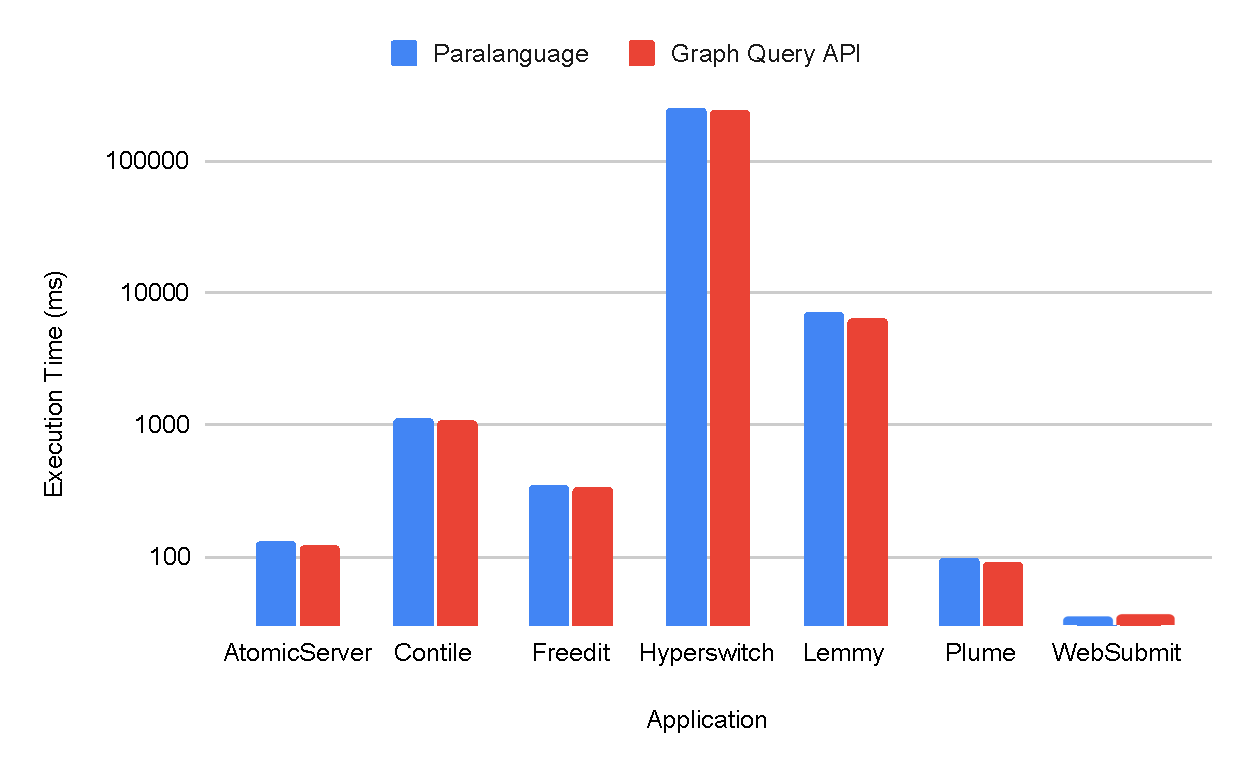
\includegraphics[scale=0.7]{graphics/times.pdf}
        \caption{\syslang{} and Graph Query policy execution times, averaged across 10 runs.}
        \label{f:times}
    \end{centering}
\end{figure}
%
\begin{figure}
    \begin{tabular}{|l|p{3cm}|p{3.5cm}|p{2cm}|p{3cm}|}
        \hline
        \textbf{Application} & \textbf{\syslang{} Time (ms)} & \textbf{Graph Query API Time (ms)} & \textbf{Difference (ms)} & \textbf{\syslang{} \% Slower} \\ \hline
        AtomicServer & 127.92    & 118.8     & 9.12    & 7.68  \\ \hline
        Contile      & 1109.14   & 1064.43   & 44.71   & 4.2   \\ \hline
        Freedit      & 347.57    & 339.85    & 7.72    & 2.27  \\ \hline
        Hyperswitch  & 251044.37 & 241890.42 & 9153.95 & 3.78  \\ \hline
        Lemmy        & 7026.23   & 6277.3    & 748.93  & 11.93 \\ \hline
        Plume        & 95.63     & 88.86     & 6.77    & 7.62  \\ \hline
        WebSubmit    & 29.89     & 30.07     & -0.18   & -0.6  \\ \hline               
        \end{tabular}
        \caption{Comparison of \syslang{} and Graph Query API policy execution times.}
        \label{f:percentages}
\end{figure}
%
These results demonstrate that \syslang{} policies incur an acceptable overhead compared to native Rust policies.
